\documentclass[]{article}
\usepackage{lmodern}
\usepackage{amssymb,amsmath}
\usepackage{ifxetex,ifluatex}
\usepackage{fixltx2e} % provides \textsubscript
\ifnum 0\ifxetex 1\fi\ifluatex 1\fi=0 % if pdftex
  \usepackage[T1]{fontenc}
  \usepackage[utf8]{inputenc}
\else % if luatex or xelatex
  \ifxetex
    \usepackage{mathspec}
    \usepackage{xltxtra,xunicode}
  \else
    \usepackage{fontspec}
  \fi
  \defaultfontfeatures{Mapping=tex-text,Scale=MatchLowercase}
  \newcommand{\euro}{€}
\fi
% use upquote if available, for straight quotes in verbatim environments
\IfFileExists{upquote.sty}{\usepackage{upquote}}{}
% use microtype if available
\IfFileExists{microtype.sty}{%
\usepackage{microtype}
\UseMicrotypeSet[protrusion]{basicmath} % disable protrusion for tt fonts
}{}
\ifxetex
  \usepackage[setpagesize=false, % page size defined by xetex
              unicode=false, % unicode breaks when used with xetex
              xetex]{hyperref}
\else
  \usepackage[unicode=true]{hyperref}
\fi
\hypersetup{breaklinks=true,
            bookmarks=true,
            pdfauthor={Metrum Research Group, LLC},
            pdftitle={Introduction to Bayesian pharmacometric data analysis using NONMEM},
            colorlinks=true,
            citecolor=blue,
            urlcolor=blue,
            linkcolor=magenta,
            pdfborder={0 0 0}}
\urlstyle{same}  % don't use monospace font for urls
\usepackage{color}
\usepackage{fancyvrb}
\newcommand{\VerbBar}{|}
\newcommand{\VERB}{\Verb[commandchars=\\\{\}]}
\DefineVerbatimEnvironment{Highlighting}{Verbatim}{commandchars=\\\{\}}
% Add ',fontsize=\small' for more characters per line
\usepackage{framed}
\definecolor{shadecolor}{RGB}{248,248,248}
\newenvironment{Shaded}{\begin{snugshade}}{\end{snugshade}}
\newcommand{\KeywordTok}[1]{\textcolor[rgb]{0.13,0.29,0.53}{\textbf{{#1}}}}
\newcommand{\DataTypeTok}[1]{\textcolor[rgb]{0.13,0.29,0.53}{{#1}}}
\newcommand{\DecValTok}[1]{\textcolor[rgb]{0.00,0.00,0.81}{{#1}}}
\newcommand{\BaseNTok}[1]{\textcolor[rgb]{0.00,0.00,0.81}{{#1}}}
\newcommand{\FloatTok}[1]{\textcolor[rgb]{0.00,0.00,0.81}{{#1}}}
\newcommand{\ConstantTok}[1]{\textcolor[rgb]{0.00,0.00,0.00}{{#1}}}
\newcommand{\CharTok}[1]{\textcolor[rgb]{0.31,0.60,0.02}{{#1}}}
\newcommand{\SpecialCharTok}[1]{\textcolor[rgb]{0.00,0.00,0.00}{{#1}}}
\newcommand{\StringTok}[1]{\textcolor[rgb]{0.31,0.60,0.02}{{#1}}}
\newcommand{\VerbatimStringTok}[1]{\textcolor[rgb]{0.31,0.60,0.02}{{#1}}}
\newcommand{\SpecialStringTok}[1]{\textcolor[rgb]{0.31,0.60,0.02}{{#1}}}
\newcommand{\ImportTok}[1]{{#1}}
\newcommand{\CommentTok}[1]{\textcolor[rgb]{0.56,0.35,0.01}{\textit{{#1}}}}
\newcommand{\DocumentationTok}[1]{\textcolor[rgb]{0.56,0.35,0.01}{\textbf{\textit{{#1}}}}}
\newcommand{\AnnotationTok}[1]{\textcolor[rgb]{0.56,0.35,0.01}{\textbf{\textit{{#1}}}}}
\newcommand{\CommentVarTok}[1]{\textcolor[rgb]{0.56,0.35,0.01}{\textbf{\textit{{#1}}}}}
\newcommand{\OtherTok}[1]{\textcolor[rgb]{0.56,0.35,0.01}{{#1}}}
\newcommand{\FunctionTok}[1]{\textcolor[rgb]{0.00,0.00,0.00}{{#1}}}
\newcommand{\VariableTok}[1]{\textcolor[rgb]{0.00,0.00,0.00}{{#1}}}
\newcommand{\ControlFlowTok}[1]{\textcolor[rgb]{0.13,0.29,0.53}{\textbf{{#1}}}}
\newcommand{\OperatorTok}[1]{\textcolor[rgb]{0.81,0.36,0.00}{\textbf{{#1}}}}
\newcommand{\BuiltInTok}[1]{{#1}}
\newcommand{\ExtensionTok}[1]{{#1}}
\newcommand{\PreprocessorTok}[1]{\textcolor[rgb]{0.56,0.35,0.01}{\textit{{#1}}}}
\newcommand{\AttributeTok}[1]{\textcolor[rgb]{0.77,0.63,0.00}{{#1}}}
\newcommand{\RegionMarkerTok}[1]{{#1}}
\newcommand{\InformationTok}[1]{\textcolor[rgb]{0.56,0.35,0.01}{\textbf{\textit{{#1}}}}}
\newcommand{\WarningTok}[1]{\textcolor[rgb]{0.56,0.35,0.01}{\textbf{\textit{{#1}}}}}
\newcommand{\AlertTok}[1]{\textcolor[rgb]{0.94,0.16,0.16}{{#1}}}
\newcommand{\ErrorTok}[1]{\textcolor[rgb]{0.64,0.00,0.00}{\textbf{{#1}}}}
\newcommand{\NormalTok}[1]{{#1}}
%%%\usepackage{graphicx,grffile}
%\makeatletter
%\def\maxwidth{\ifdim\Gin@nat@width>\linewidth\linewidth\else\Gin@nat@width\fi}
%\def\maxheight{\ifdim\Gin@nat@height>\textheight\textheight\else\Gin@nat@height\fi}
%\makeatother
% Scale images if necessary, so that they will not overflow the page
% margins by default, and it is still possible to overwrite the defaults
% using explicit options in \includegraphics[width, height, ...]{}
%\setkeys{Gin}{width=\maxwidth,height=\maxheight,keepaspectratio}
%%\setlength{\parindent}{0pt}
\setlength{\parskip}{6pt plus 2pt minus 1pt}
\setlength{\emergencystretch}{3em}  % prevent overfull lines
\providecommand{\tightlist}{%
  \setlength{\itemsep}{0pt}\setlength{\parskip}{0pt}}
\setcounter{secnumdepth}{5}

%%% Use protect on footnotes to avoid problems with footnotes in titles
\let\rmarkdownfootnote\footnote%
\def\footnote{\protect\rmarkdownfootnote}

%%% Change title format to be more compact
\usepackage{titling}

% Create subtitle command for use in maketitle
\newcommand{\subtitle}[1]{
  \posttitle{
    \begin{center}\large#1\end{center}
    }
}

\setlength{\droptitle}{-2em}
  \title{Introduction to Bayesian pharmacometric data analysis using NONMEM}
  \pretitle{\vspace{\droptitle}\centering\huge}
  \posttitle{\par}
  \author{Metrum Research Group, LLC}
  \preauthor{\centering\large\emph}
  \postauthor{\par}
  \predate{\centering\large\emph}
  \postdate{\par}
  \date{November 03, 2018}

\usepackage{pdfpages}
\usepackage{pdflscape}
\usepackage{graphicx}
\usepackage{geometry}
\usepackage{bm}
\usepackage{multirow}
\newcommand{\figDir}{../deliv/figure}
\newcommand{\tabDir}{../deliv/table}
\usepackage{longtable}
\usepackage{tabu}
\usepackage{fancyhdr, lastpage}

\pagestyle{fancy}


\usepackage{textpos}
\usepackage{float}
\floatplacement{figure}{H}
\floatplacement{table}{H}

% Redefines (sub)paragraphs to behave more like sections
\ifx\paragraph\undefined\else
\let\oldparagraph\paragraph
\renewcommand{\paragraph}[1]{\oldparagraph{#1}\mbox{}}
\fi
\ifx\subparagraph\undefined\else
\let\oldsubparagraph\subparagraph
\renewcommand{\subparagraph}[1]{\oldsubparagraph{#1}\mbox{}}
\fi

%%%%%%%%change date format to metrum style%%%%%%%
\usepackage{datetime}
\newcommand{\todaymetrum}{\the\year-\twodigit{\month}-\twodigit{\day}}

\usepackage{fancyhdr, lastpage}

\pagestyle{fancy}

\rhead{Project Number:\  \\Sponsor: }
\lhead{Metrum Research Group LLC\\CONFIDENTIAL}
%\rfoot{Right bottom}
%\cfoot{Page \thepage\ of \pageref{LastPage}}


\usepackage{graphicx}
\usepackage{longtable}
%better control of float; adds [H] option (to be used instead of clearpage in figures/tables sections)
\usepackage{float}
\floatplacement{figure}{H}
\floatplacement{table}{H}
\usepackage{bm}

% \newcommand{\figDir}{../deliv/figure}
% \newcommand{\tabDir}{../deliv/table}
\newcommand{\doctitle}{Introduction to Bayesian pharmacometric data analysis using NONMEM}

\newcommand{\clientname}{Client Name}
\newcommand{\clienttitle}{Client Title}
\newcommand{\companyname}{Company Name}
\newcommand{\clientstreet}{123 Street Rd.}
\newcommand{\clientcitystate}{City, State ZIP}
\newcommand{\clientcountry}{Country}
\newcommand{\clientphone}{Phone: 555-555-5555}
\newcommand{\clientfax}{Fax: 555-555-5554}
\newcommand{\clientemail}{name@domain.com}

\newcommand{\scientist}{Metrum Research Group, LLC}
\newcommand{\scientistphone}{Phone: 860-735-7043}
\newcommand{\scientistfax}{Fax: 860-760-6014}


\rhead{Project Number:  \\Sponsor: }
\lhead{Metrum Research Group LLC\\CONFIDENTIAL}
%\rfoot{Right bottom}
%\cfoot{Page \thepage\ of \pageref{LastPage}}


\begin{document}
%\maketitle
\begin{center}

\includegraphics[scale=.7]{mrglogo.pdf}
\vspace{1cm}

{\Large CONFIDENTIAL}
\vspace{3.0cm}

{\huge \doctitle}
\vspace{1cm}

\todaymetrum
\vspace{6cm}

{\large\bfseries Author:}\\
\scientist \\
 Metrum Research Group LLC\\
Tunxis Road, Suite 112\\
Tariffville, CT 06081\\
\end{center}


\newpage



{
\hypersetup{linkcolor=black}
\setcounter{tocdepth}{2}
\tableofcontents
}
\section{Population Parameter
Estimation}\label{population-parameter-estimation}

\subsection{Estimation of pediatric atorvastatin PK given informative
priors based on
adults}\label{estimation-of-pediatric-atorvastatin-pk-given-informative-priors-based-on-adults}

\begin{figure}[htbp]
\centering
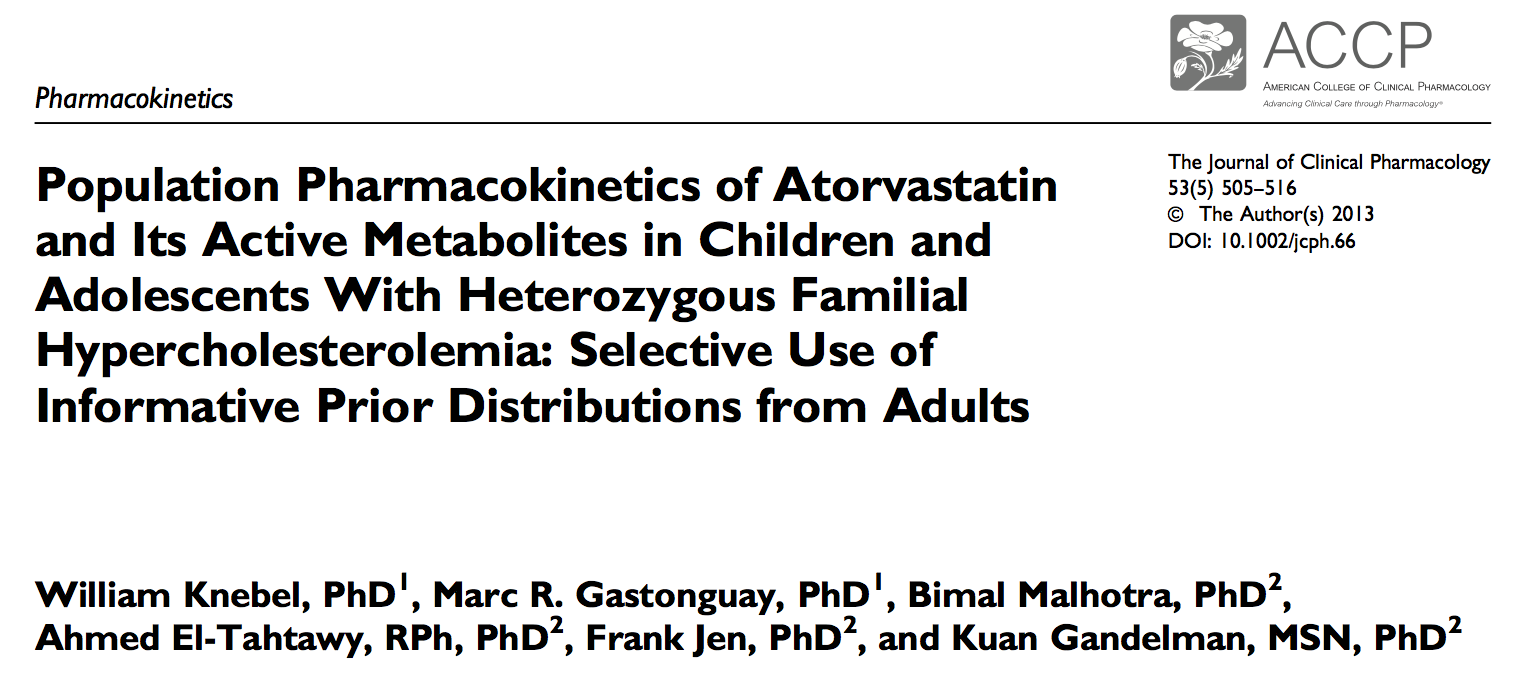
\includegraphics{../doc/IntroBayesNONMEMMerck14Nov2018/graphics/KnebelTitle.png}
\caption{}
\end{figure}

\begin{center}\rule{0.5\linewidth}{\linethickness}\end{center}

\begin{figure}[htbp]
\centering
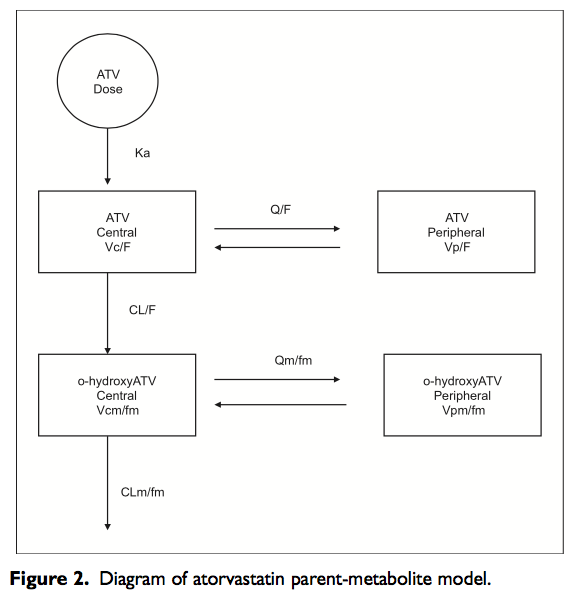
\includegraphics{../doc/IntroBayesNONMEMMerck14Nov2018/graphics/KnebelModel.png}
\caption{}
\end{figure}

\begin{center}\rule{0.5\linewidth}{\linethickness}\end{center}

\subsection{Specification of prior distributions for population means
and inter-individual
covariance}\label{specification-of-prior-distributions-for-population-means-and-inter-individual-covariance}

\subsection{\texorpdfstring{\protect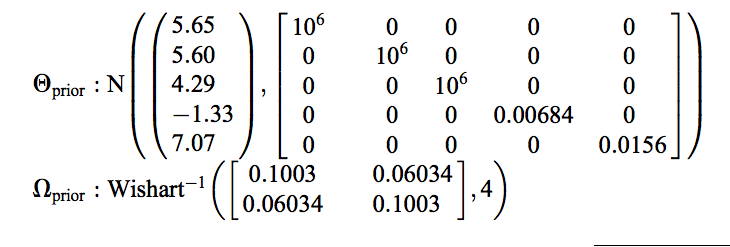
\includegraphics{../doc/IntroBayesNONMEMMerck14Nov2018/graphics/KnebelPrior.png}}{}}\label{section}

\subsection{Setup R environment}\label{setup-r-environment}

\begin{Shaded}
\begin{Highlighting}[]
\KeywordTok{rm}\NormalTok{(}\DataTypeTok{list =} \KeywordTok{ls}\NormalTok{())}
\KeywordTok{gc}\NormalTok{()}

\NormalTok{knitr::opts_chunk$}\KeywordTok{set}\NormalTok{(}
  \DataTypeTok{comment =} \StringTok{'.'}\NormalTok{, }
  \DataTypeTok{fig.height =} \DecValTok{5}\NormalTok{, }
  \DataTypeTok{fig.width =} \DecValTok{9}\NormalTok{,}
  \DataTypeTok{eval.after =} \StringTok{'fig.cap'}\NormalTok{,}
  \DataTypeTok{message =} \OtherTok{FALSE}
\NormalTok{)}

\NormalTok{modelName <-}\StringTok{ "atorv1"}
\NormalTok{scriptName <-}\StringTok{ }\KeywordTok{paste}\NormalTok{(modelName, }\StringTok{"Rmd"}\NormalTok{, }\DataTypeTok{sep =} \StringTok{"."}\NormalTok{)}
\NormalTok{fitModel <-}\StringTok{ }\OtherTok{FALSE}

\NormalTok{## Relative paths assuming the working directory is the script directory}
\NormalTok{## containing this script}
\NormalTok{scriptDir <-}\StringTok{ }\KeywordTok{getwd}\NormalTok{()}
\NormalTok{projectDir <-}\StringTok{ }\KeywordTok{dirname}\NormalTok{(scriptDir)}
\NormalTok{dataDir <-}\StringTok{ }\KeywordTok{file.path}\NormalTok{(projectDir, }\StringTok{"data"}\NormalTok{)}
\NormalTok{modelDir <-}\StringTok{ }\KeywordTok{file.path}\NormalTok{(projectDir, }\StringTok{"model"}\NormalTok{)}
\NormalTok{outDir <-}\StringTok{ }\KeywordTok{file.path}\NormalTok{(modelDir, modelName)}
\NormalTok{figDir <-}\StringTok{ }\KeywordTok{file.path}\NormalTok{(projectDir, }\StringTok{"deliv"}\NormalTok{, }\StringTok{"figure"}\NormalTok{, modelName)}
\NormalTok{tabDir <-}\StringTok{ }\KeywordTok{file.path}\NormalTok{(projectDir, }\StringTok{"deliv"}\NormalTok{, }\StringTok{"table"}\NormalTok{, modelName)}
\KeywordTok{invisible}\NormalTok{(}\KeywordTok{dir.create}\NormalTok{(figDir, }\DataTypeTok{recursive =} \OtherTok{TRUE}\NormalTok{))}
\end{Highlighting}
\end{Shaded}

\begin{verbatim}
## Warning in dir.create(figDir, recursive = TRUE): '/data/IntroBayesNONMEM/
## deliv/figure/atorv1' already exists
\end{verbatim}

\begin{Shaded}
\begin{Highlighting}[]
\KeywordTok{invisible}\NormalTok{(}\KeywordTok{dir.create}\NormalTok{(tabDir, }\DataTypeTok{recursive =} \OtherTok{TRUE}\NormalTok{))}
\end{Highlighting}
\end{Shaded}

\begin{verbatim}
## Warning in dir.create(tabDir, recursive = TRUE): '/data/IntroBayesNONMEM/
## deliv/table/atorv1' already exists
\end{verbatim}

\begin{Shaded}
\begin{Highlighting}[]
\NormalTok{knitr::opts_chunk$}\KeywordTok{set}\NormalTok{(}
  \DataTypeTok{fig.path =} \KeywordTok{file.path}\NormalTok{(figDir, }\KeywordTok{paste}\NormalTok{(modelName, }\StringTok{"_"}\NormalTok{, }\DataTypeTok{sep =} \StringTok{""}\NormalTok{))}
\NormalTok{)}

\KeywordTok{.libPaths}\NormalTok{(}\StringTok{"lib"}\NormalTok{)}

\KeywordTok{library}\NormalTok{(metrumrg)}
\end{Highlighting}
\end{Shaded}

\begin{verbatim}
## Loading required package: reshape
\end{verbatim}

\begin{verbatim}
## Loading required package: lattice
\end{verbatim}

\begin{verbatim}
## Loading required package: XML
\end{verbatim}

\begin{verbatim}
## Loading required package: MASS
\end{verbatim}

\begin{verbatim}
## Loading required package: grid
\end{verbatim}

\begin{verbatim}
## metrumrg 5.57
\end{verbatim}

\begin{verbatim}
## enter "?metrumrg" for help
\end{verbatim}

\begin{Shaded}
\begin{Highlighting}[]
\KeywordTok{suppressMessages}\NormalTok{(}\KeywordTok{library}\NormalTok{(rstan))}
\KeywordTok{suppressMessages}\NormalTok{(}\KeywordTok{library}\NormalTok{(bayesplot))}
\KeywordTok{suppressMessages}\NormalTok{(}\KeywordTok{library}\NormalTok{(tidyverse))}
\KeywordTok{library}\NormalTok{(gridExtra)}
\end{Highlighting}
\end{Shaded}

\begin{verbatim}
## 
## Attaching package: 'gridExtra'
\end{verbatim}

\begin{verbatim}
## The following object is masked from 'package:dplyr':
## 
##     combine
\end{verbatim}

\begin{Shaded}
\begin{Highlighting}[]
\KeywordTok{library}\NormalTok{(kableExtra)}
\KeywordTok{library}\NormalTok{(parallel)}
\KeywordTok{library}\NormalTok{(knitr)}
\KeywordTok{library}\NormalTok{(qapply)}
\end{Highlighting}
\end{Shaded}

\begin{verbatim}
## Loading required package: rlecuyer
\end{verbatim}

\begin{verbatim}
## 
## Attaching package: 'qapply'
\end{verbatim}

\begin{verbatim}
## The following object is masked from 'package:metrumrg':
## 
##     qstat
\end{verbatim}

\begin{Shaded}
\begin{Highlighting}[]
\KeywordTok{library}\NormalTok{(PKPDmisc)}

\NormalTok{## Go back to default ggplot2 theme that was overridden by bayesplot}
\KeywordTok{theme_set}\NormalTok{(}\KeywordTok{theme_gray}\NormalTok{())}

\KeywordTok{source}\NormalTok{(}\KeywordTok{file.path}\NormalTok{(scriptDir, }\StringTok{"tools"}\NormalTok{, }\StringTok{"stanTools2.R"}\NormalTok{))}
\KeywordTok{source}\NormalTok{(}\KeywordTok{file.path}\NormalTok{(scriptDir, }\StringTok{"tools"}\NormalTok{, }\StringTok{"functions.R"}\NormalTok{))}

\KeywordTok{rstan_options}\NormalTok{(}\DataTypeTok{auto_write =} \OtherTok{TRUE}\NormalTok{)}
\KeywordTok{options}\NormalTok{(}\DataTypeTok{mc.cores =} \NormalTok{parallel::}\KeywordTok{detectCores}\NormalTok{())}

\KeywordTok{set.seed}\NormalTok{(}\DecValTok{11191951}\NormalTok{) }
\end{Highlighting}
\end{Shaded}

\subsection{The NONMEM model stub}\label{the-nonmem-model-stub}

\begin{Shaded}
\begin{Highlighting}[]
\NormalTok{modelFile <-}\StringTok{ }\KeywordTok{file.path}\NormalTok{(modelDir, }\KeywordTok{paste}\NormalTok{(modelName, }\StringTok{"stub.ctl"}\NormalTok{, }\DataTypeTok{sep =} \StringTok{""}\NormalTok{))}
\NormalTok{modelText <-}\StringTok{ }\KeywordTok{readLines}\NormalTok{(modelFile)}
\KeywordTok{cat}\NormalTok{(modelText, }\DataTypeTok{sep =} \StringTok{"}\CharTok{\textbackslash{}n}\StringTok{"}\NormalTok{)}
\end{Highlighting}
\end{Shaded}

\begin{verbatim}
. $PROBLEM RUN# atorv1 ; like 237
. $INPUT C ID SID=DROP STDY=DROP TIME DV DVR=DROP DVC=DROP AMT AMTO=DROP CMT TYPE=DROP
.        DOSE DOSN=DROP NTIM=DROP EVID MDV ADDL II SS FORM WT SEX=DROP AGE
.        HT=DROP RACE=DROP PER BLQ TRCD=DROP ANLT=DROP TXT=DROP 
. $DATA ../../../data/atorv1172atvb.csv IGNORE=(C='C', BLQ.EQ.1)
. 
. $ABBR DECLARE INTEGER FIRST_WRITE_PAR
. $ABBR DECLARE INTEGER FIRST_WRITE_IPAR
. ;$ABBR DECLARE INTEGER FIRST_WRITE_IPRED
. 
. $SUBROUTINES ADVAN4 TRANS4
. 
. $PK
. ; Request extra information for Bayesian analysis.
. ; An extra call will then be made for accepted samples 
. include '/opt/NONMEM/nm74/util/nonmem_reserved_general'
. BAYES_EXTRA_REQUEST=1
. 
. MU_1 = THETA(1)     
. MU_2 = THETA(2) 
. 
. VWT = LOG(WT/70) ; normalized to 70 kg adult
. 
. ;ATORVASTATIN
. 
. CL = EXP(MU_1+(VWT*0.75)+ETA(1)) ; atv cl 
. V2 = EXP(MU_2+VWT+ETA(2))
. LNQ = THETA(3);+(VWT*0.75)
. Q = EXP(LNQ)
. LNV3 = THETA(5)+VWT
. V3 = EXP(LNV3)
. 
. LNKA = THETA(4)   
. KA = EXP(LNKA)
. S2 = V2/1000              ; DOSE IN uM & CONC IN nM/L
. F1 = 1.0             ; TABLET AS REFERENCE
. IF(FORM.EQ.2) F1 = THETA(6)  ; CHEWABLE F1
. 
. IF(BAYES_EXTRA==1 .AND. NIREC==1 .AND. NDREC==1 .AND. &
.    ITER_REPORT>0) THEN 
.   IF(FIRST_WRITE_PAR==0) THEN
.     " OPEN(unit=52,FILE='./par.txt') 
.     FIRST_WRITE_PAR=1
.   ENDIF
.   " WRITE(52,'(I12,1X,20(1X,1PG19.10E3))') ITER_REPORT, &  
.   " OMEGA(1,1), OMEGA(2,1), OMEGA(2,2), &
.   " THETA(1), THETA(2), THETA(3), THETA(4), THETA(5), THETA(6), THETA(7)
. ENDIF
. IF(BAYES_EXTRA==1 .AND. NDREC==1 .AND. ITER_REPORT>0) THEN 
.   IF(FIRST_WRITE_IPAR==0) THEN
.     " OPEN(unit=50,FILE='./ipar'//TFI(PNM_NODE_NUMBER)//'.txt') 
.     FIRST_WRITE_IPAR=1
.   ENDIF
.   " WRITE(50,'(I12,1X,F14.0,10(1X,1PG19.10E3))') ITER_REPORT, ID, KA, CL, V2, Q, V3, F1
. ENDIF
. 
. 
. $ERROR
. 
. ;    TYPE          ANLT 
. ;       1    atorvastatin 
. ;       2    o-hydroxy atv 
. ;       3    p-hydroxy atv
. 
. TYP=1
. SIG1=EXP(THETA(7))
. LOQ = 0.45          ; nM/L
. IPRED = F
. DUM = (LOQ-IPRED)/(SIG1*IPRED)
. CUMD=PHI(DUM)
. IF(BLQ.EQ.0)THEN
.   F_FLAG=0
.   Y = F*(1+SIG1*ERR(1)) ; ATV
.   TTV = F_FLAG
. ELSE
.   F_FLAG=1
.   Y=CUMD
. ENDIF
. 
. ; Code below into chains
\end{verbatim}

\subsection{Assemble initial estimates, priors and table
specs}\label{assemble-initial-estimates-priors-and-table-specs}

\begin{Shaded}
\begin{Highlighting}[]
\NormalTok{## create initial estimates}
\NormalTok{geninit <-}\StringTok{ }\NormalTok{function()\{}
    \KeywordTok{paste}\NormalTok{(}\KeywordTok{c}\NormalTok{(}
    \StringTok{"; Initial values of THETA"}\NormalTok{,}
    \StringTok{"$THETA"}\NormalTok{,}
    \KeywordTok{paste}\NormalTok{(}\KeywordTok{rnorm}\NormalTok{(}\DecValTok{1}\NormalTok{, }\FloatTok{6.0}\NormalTok{,}\FloatTok{1.0}\NormalTok{), }\StringTok{"     ; TOTAL CL ATV = THETA(1)"}\NormalTok{),}
    \KeywordTok{paste}\NormalTok{(}\KeywordTok{rnorm}\NormalTok{(}\DecValTok{1}\NormalTok{, }\FloatTok{6.0}\NormalTok{, }\FloatTok{1.0}\NormalTok{), }\StringTok{"     ; V2 = THETA(2)"}\NormalTok{),}
    \KeywordTok{paste}\NormalTok{(}\KeywordTok{rnorm}\NormalTok{(}\DecValTok{1}\NormalTok{, }\FloatTok{5.0}\NormalTok{,}\FloatTok{1.0}\NormalTok{), }\StringTok{"   ; Q = THETA(3)"}\NormalTok{),}
    \KeywordTok{paste}\NormalTok{(}\KeywordTok{rnorm}\NormalTok{(}\DecValTok{1}\NormalTok{, -}\FloatTok{1.5}\NormalTok{, }\FloatTok{0.5}\NormalTok{), }\StringTok{"   ; KA= THETA(4) "}\NormalTok{),}
    \KeywordTok{paste}\NormalTok{(}\KeywordTok{rnorm}\NormalTok{(}\DecValTok{1}\NormalTok{, }\FloatTok{7.4}\NormalTok{, }\FloatTok{1.0}\NormalTok{), }\StringTok{"   ; V3 = THETA(5) "}\NormalTok{),}
    \StringTok{"(0,1) ; THETA(6) relative F1 CHEWABLE"}\NormalTok{,}
    \StringTok{"(-3.2189) ; THETA(7) - PRO RES ERROR"}\NormalTok{,   }\CommentTok{# equiv. to initial 0.04 on a linear scale}
    \StringTok{"$OMEGA BLOCK(2) ;INITIAL values of OMEGAs"}\NormalTok{,}
    \StringTok{"0.1           ; cl"}\NormalTok{,}
    \StringTok{"0.03  0.2     ; v2"}\NormalTok{,}
    \StringTok{"$SIGMA  ;Initial value of SIGMA"}\NormalTok{,}
    \StringTok{"1 FIX; pro"}\NormalTok{),}
    \DataTypeTok{sep =} \StringTok{"}\CharTok{\textbackslash{}n}\StringTok{"}\NormalTok{)}
\NormalTok{\}}

\NormalTok{## Set parameters of the prior distribution}
\NormalTok{priors <-}\StringTok{ }\KeywordTok{paste}\NormalTok{(}\KeywordTok{c}\NormalTok{(}\StringTok{"$PRIOR NWPRI"}\NormalTok{,}
                  \StringTok{"$THETAP          ; Prior information of THETAS"}\NormalTok{,}
                  \StringTok{"(5.65 FIX)      ;  THETA(1) TOTAL CL ATV"}\NormalTok{,}
                  \StringTok{"(5.60 FIX)      ;  THETA(2) V2"}\NormalTok{,}
                  \StringTok{"(4.29 FIX)      ;  THETA(3) Q"}\NormalTok{,}
                  \StringTok{"(-1.33 FIX)      ; THETA(4) KA"}\NormalTok{,}
                  \StringTok{"(7.07 FIX)      ;  THETA(5) V3"}\NormalTok{,}
                  \StringTok{"$THETAPV BLOCK(5)     ;  variances for priors on THETAS (var-cov)"}\NormalTok{,}
                  \StringTok{"12 FIX ; CL uninformative"}\NormalTok{,}
                  \StringTok{"0.00 12  ; V2 SE**2 FROM CADUET"}\NormalTok{,}
                  \StringTok{"0.00 0.00 12  ; Q SE**2 FROM CADUET"}\NormalTok{,}
                  \StringTok{"0.00 0.00 0.00 .00684   ; KA SE**2 FROM CADUET range of ka based on dose"}\NormalTok{,}
                  \StringTok{"0.00 0.00 0.00 0.00 .0156    ; SE**2 of V2 FROM CADUET since no V3 estimate"}\NormalTok{,}
                  \StringTok{"$OMEGAP BLOCK(2)   ; prior information for OMEGA - FROM CADUET"}\NormalTok{,}
                  \StringTok{".1003   FIXED         ; cl"}\NormalTok{,}
                  \StringTok{".06034    .8477       ; v2"}\NormalTok{,}
                  \StringTok{"$OMEGAPD (4.0, FIXED)     ; df for OMEGA prior"}
\NormalTok{),}
\DataTypeTok{sep =} \StringTok{"}\CharTok{\textbackslash{}n}\StringTok{"}\NormalTok{)}

\NormalTok{## Table statements}
\NormalTok{tables <-}\StringTok{ }\KeywordTok{paste}\NormalTok{(}\KeywordTok{c}\NormalTok{(}\StringTok{"$TABLE ID EVID TIME DV IPRED CWRES CWRESI NPDE AGE WT"}\NormalTok{,}
                  \StringTok{"NOPRINT ONEHEADER FILE=./.tab"}\NormalTok{,}
                  \StringTok{"$TABLE ID WT CL V2 Q KA V3 ETA1 ETA2 PER FORM"}\NormalTok{,}
                  \StringTok{"NOPRINT ONEHEADER FILE=./par.tab"}\NormalTok{),}
                \DataTypeTok{sep =} \StringTok{"}\CharTok{\textbackslash{}n}\StringTok{"}\NormalTok{)}
\end{Highlighting}
\end{Shaded}

\subsection{Run NONMEM}\label{run-nonmem}

\begin{Shaded}
\begin{Highlighting}[]
\NormalTok{nChains <-}\StringTok{ }\DecValTok{4}
\NormalTok{nPost <-}\StringTok{ }\DecValTok{500} \NormalTok{## Number of post-burn-in samples per chain after thinning}
\NormalTok{nBurn <-}\StringTok{ }\DecValTok{500} \NormalTok{## Number of burn-in samples per chain after thinning}
\NormalTok{nThin <-}\StringTok{ }\DecValTok{10}

\NormalTok{seed =}\StringTok{ }\KeywordTok{sample}\NormalTok{(}\DecValTok{10000}\NormalTok{, }\DataTypeTok{size =} \NormalTok{nChains)}
\NormalTok{if(fitModel)\{}
  \NormalTok{if(!}\KeywordTok{file.exists}\NormalTok{(}\KeywordTok{file.path}\NormalTok{(modelDir, modelName))) }
    \KeywordTok{dir.create}\NormalTok{(}\KeywordTok{file.path}\NormalTok{(modelDir, modelName))}
  \NormalTok{runChains <-}\StringTok{ }\KeywordTok{lapply}\NormalTok{(}\DecValTok{1}\NormalTok{:nChains, runChain,}
                      \DataTypeTok{modelName =} \NormalTok{modelName, }\DataTypeTok{modelDir =} \NormalTok{modelDir, }
                      \DataTypeTok{priors =} \NormalTok{priors, }\DataTypeTok{tables =} \NormalTok{tables,}
                      \DataTypeTok{nPost =} \NormalTok{nPost, }\DataTypeTok{nBurn =} \NormalTok{nBurn, }\DataTypeTok{nThin =} \NormalTok{nThin, }
                      \DataTypeTok{seed =} \NormalTok{seed, }\DataTypeTok{print =} \DecValTok{100}\NormalTok{,}
                      \DataTypeTok{OLKJDF =} \DecValTok{0}\NormalTok{, }\DataTypeTok{OVARF =} \DecValTok{1}\NormalTok{, }\DataTypeTok{AUTO =} \DecValTok{2}\NormalTok{,}
                      \DataTypeTok{method =} \StringTok{"BAYES"}\NormalTok{, }\DataTypeTok{pe =} \StringTok{"orte 16"}\NormalTok{,}
                      \DataTypeTok{mode =} \StringTok{"para"}\NormalTok{)}
  \KeywordTok{NONR}\NormalTok{(}\DataTypeTok{run =} \KeywordTok{paste}\NormalTok{(modelName, }\StringTok{"."}\NormalTok{, }\DecValTok{1}\NormalTok{, }\DataTypeTok{sep =} \StringTok{""}\NormalTok{),}
         \DataTypeTok{command =} \StringTok{"/opt/NONMEM/nm74/nmqual/autolog.pl"}\NormalTok{,}
         \DataTypeTok{project =} \KeywordTok{file.path}\NormalTok{(modelDir, modelName),}
         \DataTypeTok{grid =} \OtherTok{FALSE}\NormalTok{,}
         \DataTypeTok{wait =} \OtherTok{FALSE}\NormalTok{,}
         \DataTypeTok{diag =} \OtherTok{FALSE}\NormalTok{,}
         \DataTypeTok{fdata =} \OtherTok{FALSE}\NormalTok{,}
         \DataTypeTok{purge =} \OtherTok{FALSE}\NormalTok{,}
         \DataTypeTok{checkrunno =} \OtherTok{TRUE}\NormalTok{)}
  
  \NormalTok{\}}
\end{Highlighting}
\end{Shaded}

\subsection{read in data file}\label{read-in-data-file}

\begin{Shaded}
\begin{Highlighting}[]
\NormalTok{dataFile <-}\StringTok{ "atorv1172atvb.csv"}
\NormalTok{nmData <-}\StringTok{ }\KeywordTok{read.csv}\NormalTok{(}\KeywordTok{file.path}\NormalTok{(dataDir, dataFile), }\DataTypeTok{as.is =} \OtherTok{TRUE}\NormalTok{)}
\end{Highlighting}
\end{Shaded}

\subsection{Get population parameters}\label{get-population-parameters}

\begin{Shaded}
\begin{Highlighting}[]
\NormalTok{## Read in posterior distributions by chain and add a column called chain}
\NormalTok{chains <-}\StringTok{ }\DecValTok{1}\NormalTok{:nChains}
\NormalTok{popParameters =}\StringTok{ }\KeywordTok{map}\NormalTok{(chains, function(thisChain)\{}
  \NormalTok{param <-}\StringTok{ }\NormalTok{data.table::}\KeywordTok{fread}\NormalTok{(}\KeywordTok{file.path}\NormalTok{(modelDir, modelName, }\KeywordTok{paste}\NormalTok{(modelName, }\StringTok{"."}\NormalTok{, thisChain, }\DataTypeTok{sep =} \StringTok{""}\NormalTok{), }
                                       \StringTok{"par.txt"}\NormalTok{), }\DataTypeTok{data.table =} \OtherTok{FALSE}\NormalTok{) }
\NormalTok{##  names(param) <- c("iteration", "V3", "Q", "SIGMA", "OMEGA(1,1)", "OMEGA(2,1)", "OMEGA(2,2)",}
\NormalTok{##                    "THETA(1)", "THETA(2)", "THETA(3)", "THETA(4)", "THETA(5)", }
\NormalTok{##                    "THETA(6)", "THETA(7)", "THETA(8)")}
  \KeywordTok{names}\NormalTok{(param) <-}\StringTok{ }\KeywordTok{c}\NormalTok{(}\StringTok{"iteration"}\NormalTok{, }\StringTok{"OMEGA11"}\NormalTok{, }\StringTok{"OMEGA21"}\NormalTok{, }\StringTok{"OMEGA22"}\NormalTok{,}
                    \StringTok{"THETA1"}\NormalTok{, }\StringTok{"THETA2"}\NormalTok{, }\StringTok{"THETA3"}\NormalTok{, }\StringTok{"THETA4"}\NormalTok{, }\StringTok{"THETA5"}\NormalTok{, }
                    \StringTok{"THETA6"}\NormalTok{, }\StringTok{"THETA7"}\NormalTok{)}
  \NormalTok{param %>%}\StringTok{ }\KeywordTok{mutate}\NormalTok{(}\DataTypeTok{chain =} \NormalTok{thisChain)}
\NormalTok{\}) %>%}\StringTok{ }\NormalTok{bind_rows}

\NormalTok{## Convert to 3-D array with dims = \{iterations, chains, parameters\}. }
\NormalTok{popParArray <-}\StringTok{ }\KeywordTok{array}\NormalTok{(}\KeywordTok{double}\NormalTok{(nPost *}\StringTok{ }\NormalTok{nChains *}\StringTok{ }\NormalTok{(}\KeywordTok{ncol}\NormalTok{(popParameters) -}\StringTok{ }\DecValTok{2}\NormalTok{)), }
                     \DataTypeTok{dim =} \KeywordTok{c}\NormalTok{(nPost, nChains, }\KeywordTok{ncol}\NormalTok{(popParameters) -}\StringTok{ }\DecValTok{2}\NormalTok{), }
                     \DataTypeTok{dimnames =}  \KeywordTok{list}\NormalTok{(}\OtherTok{NULL}\NormalTok{, }\OtherTok{NULL}\NormalTok{, }\KeywordTok{setdiff}\NormalTok{(}\KeywordTok{names}\NormalTok{(popParameters), }\KeywordTok{c}\NormalTok{(}\StringTok{"chain"}\NormalTok{, }\StringTok{"iteration"}\NormalTok{))))}
\NormalTok{for(thisChain in chains)\{}
  \NormalTok{popParArray[,thisChain,] <-}\StringTok{ }\NormalTok{popParameters %>%}
\StringTok{    }\KeywordTok{filter}\NormalTok{(chain ==}\StringTok{ }\NormalTok{thisChain,}
           \NormalTok{iteration >}\StringTok{ }\DecValTok{0}\NormalTok{) %>%}
\StringTok{    }\KeywordTok{select}\NormalTok{(-chain, -iteration) %>%}
\StringTok{    }\NormalTok{as.matrix}
\NormalTok{\}}
\end{Highlighting}
\end{Shaded}

\subsection{Get individual parameters}\label{get-individual-parameters}

\begin{Shaded}
\begin{Highlighting}[]
\NormalTok{chains <-}\StringTok{ }\DecValTok{1}\NormalTok{:nChains}
\NormalTok{indParameters =}\StringTok{ }\KeywordTok{map}\NormalTok{(chains, function(thisChain)\{}
  \NormalTok{files <-}\StringTok{ }\KeywordTok{list.files}\NormalTok{(}\KeywordTok{file.path}\NormalTok{(modelDir, modelName, }\KeywordTok{paste}\NormalTok{(modelName, }\StringTok{"."}\NormalTok{, thisChain, }\DataTypeTok{sep =} \StringTok{""}\NormalTok{)))}
  \NormalTok{iparFiles <-}\StringTok{ }\NormalTok{files[}\KeywordTok{grepl}\NormalTok{(}\StringTok{"^ipar"}\NormalTok{, files)]}
  \NormalTok{param <-}\StringTok{ }\KeywordTok{map}\NormalTok{(iparFiles, function(thisFile)\{}
    \NormalTok{data.table::}\KeywordTok{fread}\NormalTok{(}\KeywordTok{file.path}\NormalTok{(modelDir, modelName, }\KeywordTok{paste}\NormalTok{(modelName, }\StringTok{"."}\NormalTok{, thisChain, }\DataTypeTok{sep =} \StringTok{""}\NormalTok{), }
                                \NormalTok{thisFile), }\DataTypeTok{data.table =} \OtherTok{FALSE}\NormalTok{)}
  \NormalTok{\}) %>%}\StringTok{ }
\StringTok{    }\NormalTok{bind_rows }
  \KeywordTok{names}\NormalTok{(param) <-}\StringTok{ }\KeywordTok{c}\NormalTok{(}\StringTok{"iteration"}\NormalTok{, }\StringTok{"ID"}\NormalTok{, }\StringTok{"KA"}\NormalTok{, }\StringTok{"CL"}\NormalTok{, }\StringTok{"V2"}\NormalTok{, }\StringTok{"Q"}\NormalTok{, }\StringTok{"V3"}\NormalTok{, }\StringTok{"F1"}\NormalTok{)}
  \NormalTok{param %>%}\StringTok{ }\KeywordTok{mutate}\NormalTok{(}\DataTypeTok{chain =} \NormalTok{thisChain)}
\NormalTok{\}) %>%}\StringTok{ }\NormalTok{bind_rows}
\end{Highlighting}
\end{Shaded}

\subsection{MCMC diagnostics and posterior distributions of
parameters}\label{mcmc-diagnostics-and-posterior-distributions-of-parameters}

\begin{Shaded}
\begin{Highlighting}[]
\KeywordTok{options}\NormalTok{(}\DataTypeTok{bayesplot.base_size =} \DecValTok{12}\NormalTok{,}
        \DataTypeTok{bayesplot.base_family =} \StringTok{"sans"}\NormalTok{)}
\KeywordTok{color_scheme_set}\NormalTok{(}\DataTypeTok{scheme =} \StringTok{"brightblue"}\NormalTok{)}
\NormalTok{myTheme <-}\StringTok{ }\KeywordTok{theme}\NormalTok{(}\DataTypeTok{text =} \KeywordTok{element_text}\NormalTok{(}\DataTypeTok{size =} \DecValTok{12}\NormalTok{), }
                 \DataTypeTok{axis.text =} \KeywordTok{element_text}\NormalTok{(}\DataTypeTok{size =} \DecValTok{12}\NormalTok{))}

\NormalTok{plot_mcmcHistory <-}\StringTok{ }\KeywordTok{mcmcHistory}\NormalTok{(popParArray,}
                                 \DataTypeTok{nParPerPage =} \DecValTok{5}\NormalTok{, }\DataTypeTok{myTheme =} \NormalTok{myTheme)}
\NormalTok{plot_mcmcDensityByChain <-}\StringTok{ }\KeywordTok{mcmcDensity}\NormalTok{(popParArray, }
                                        \DataTypeTok{nParPerPage =} \DecValTok{16}\NormalTok{, }\DataTypeTok{byChain =} \OtherTok{TRUE}\NormalTok{, }
                                        \DataTypeTok{myTheme =} \KeywordTok{theme}\NormalTok{(}\DataTypeTok{text =} \KeywordTok{element_text}\NormalTok{(}\DataTypeTok{size =} \DecValTok{12}\NormalTok{), }
                                                        \DataTypeTok{axis.text =} \KeywordTok{element_text}\NormalTok{(}\DataTypeTok{size =} \DecValTok{10}\NormalTok{)))}
\NormalTok{plot_mcmcDensity <-}\StringTok{ }\KeywordTok{mcmcDensity}\NormalTok{(popParArray, }\DataTypeTok{nParPerPage =} \DecValTok{16}\NormalTok{, }
                                 \DataTypeTok{myTheme =} \KeywordTok{theme}\NormalTok{(}\DataTypeTok{text =} \KeywordTok{element_text}\NormalTok{(}\DataTypeTok{size =} \DecValTok{12}\NormalTok{), }
                                                 \DataTypeTok{axis.text =} \KeywordTok{element_text}\NormalTok{(}\DataTypeTok{size =} \DecValTok{10}\NormalTok{)))}

\NormalTok{plot_mcmcHistory}
\end{Highlighting}
\end{Shaded}

\begin{verbatim}
. [[1]]
\end{verbatim}

\begin{figure}[htbp]
\centering
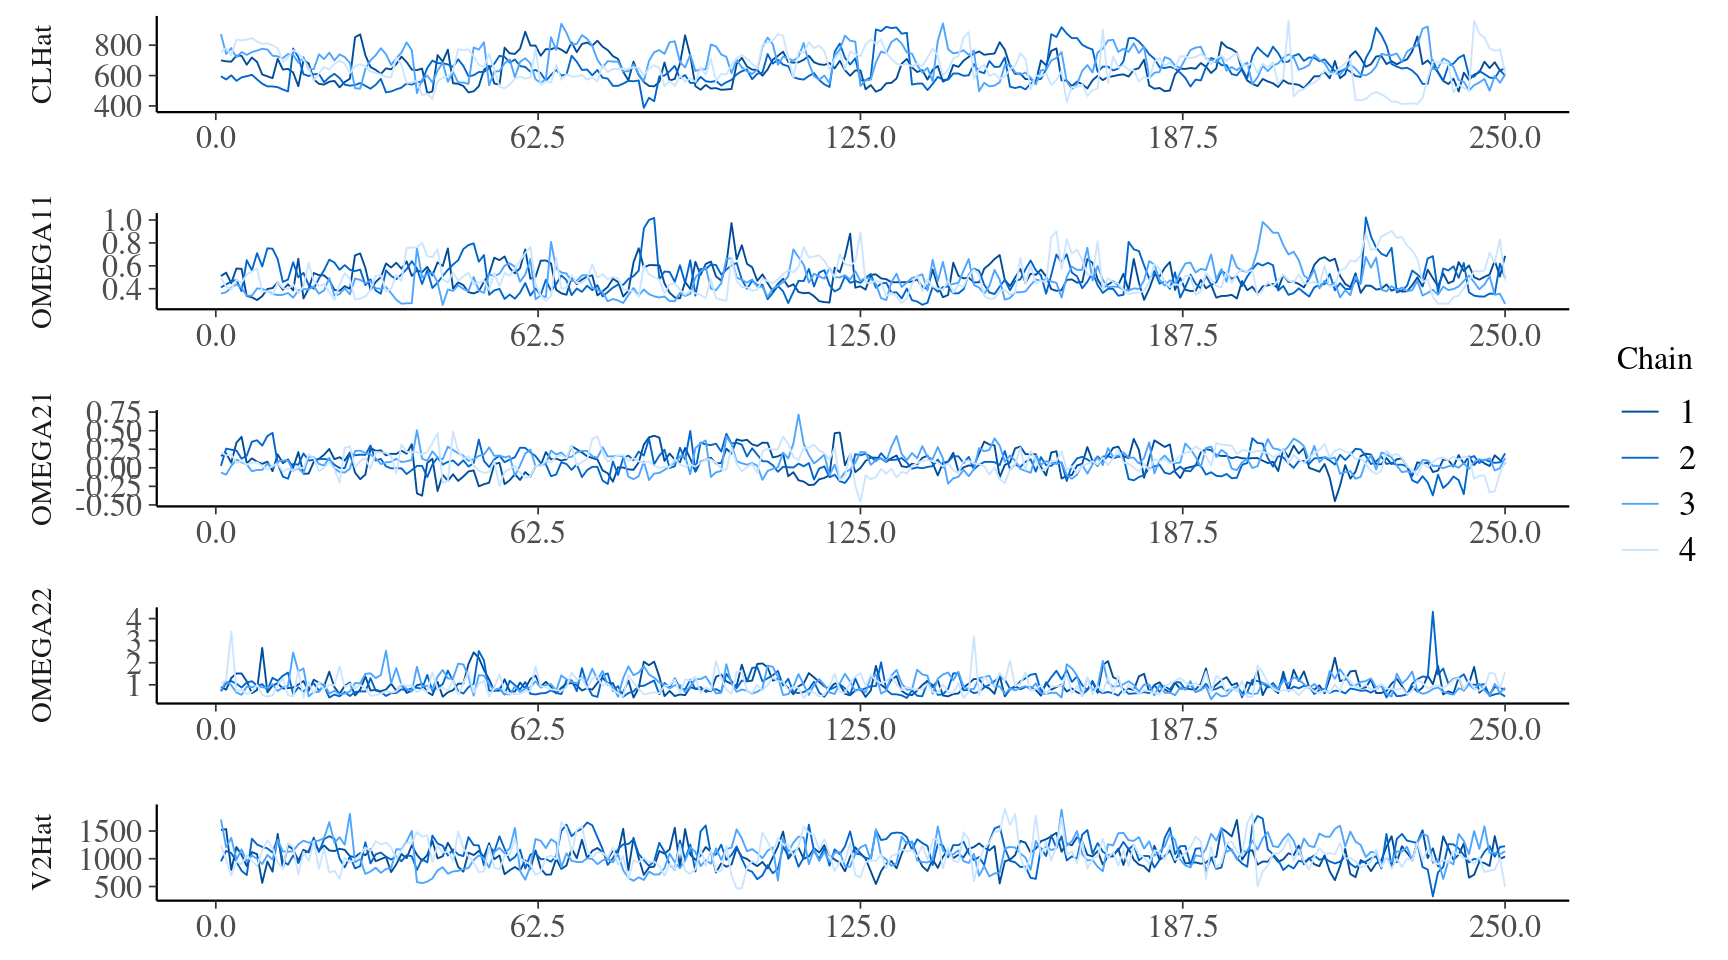
\includegraphics{/data/IntroBayesNONMEM/deliv/figure/atorv1/atorv1_parameters-1.pdf}
\caption{Pediatric atorvastatin PK example: MCMC trace plots.}
\end{figure}

\begin{verbatim}
. 
. [[2]]
\end{verbatim}

\begin{figure}[htbp]
\centering
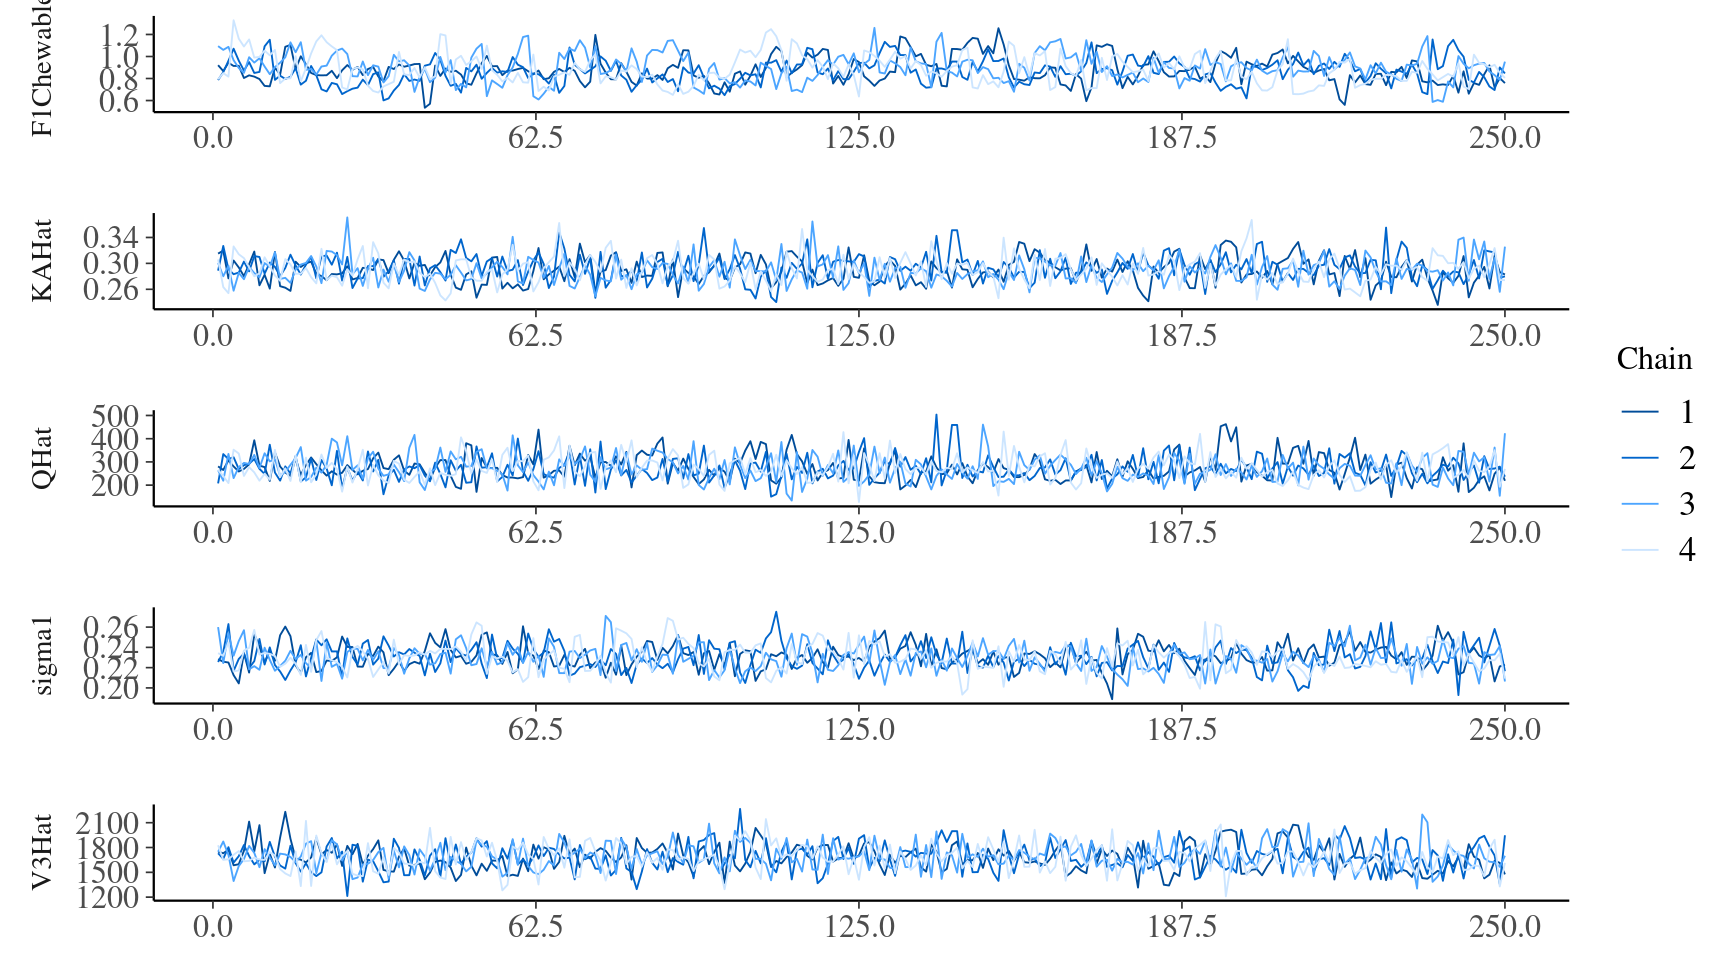
\includegraphics{/data/IntroBayesNONMEM/deliv/figure/atorv1/atorv1_parameters-2.pdf}
\caption{Pediatric atorvastatin PK example: MCMC trace plots.}
\end{figure}

\begin{Shaded}
\begin{Highlighting}[]
\NormalTok{plot_mcmcDensityByChain}
\end{Highlighting}
\end{Shaded}

\begin{verbatim}
. [[1]]
\end{verbatim}

\begin{figure}[htbp]
\centering
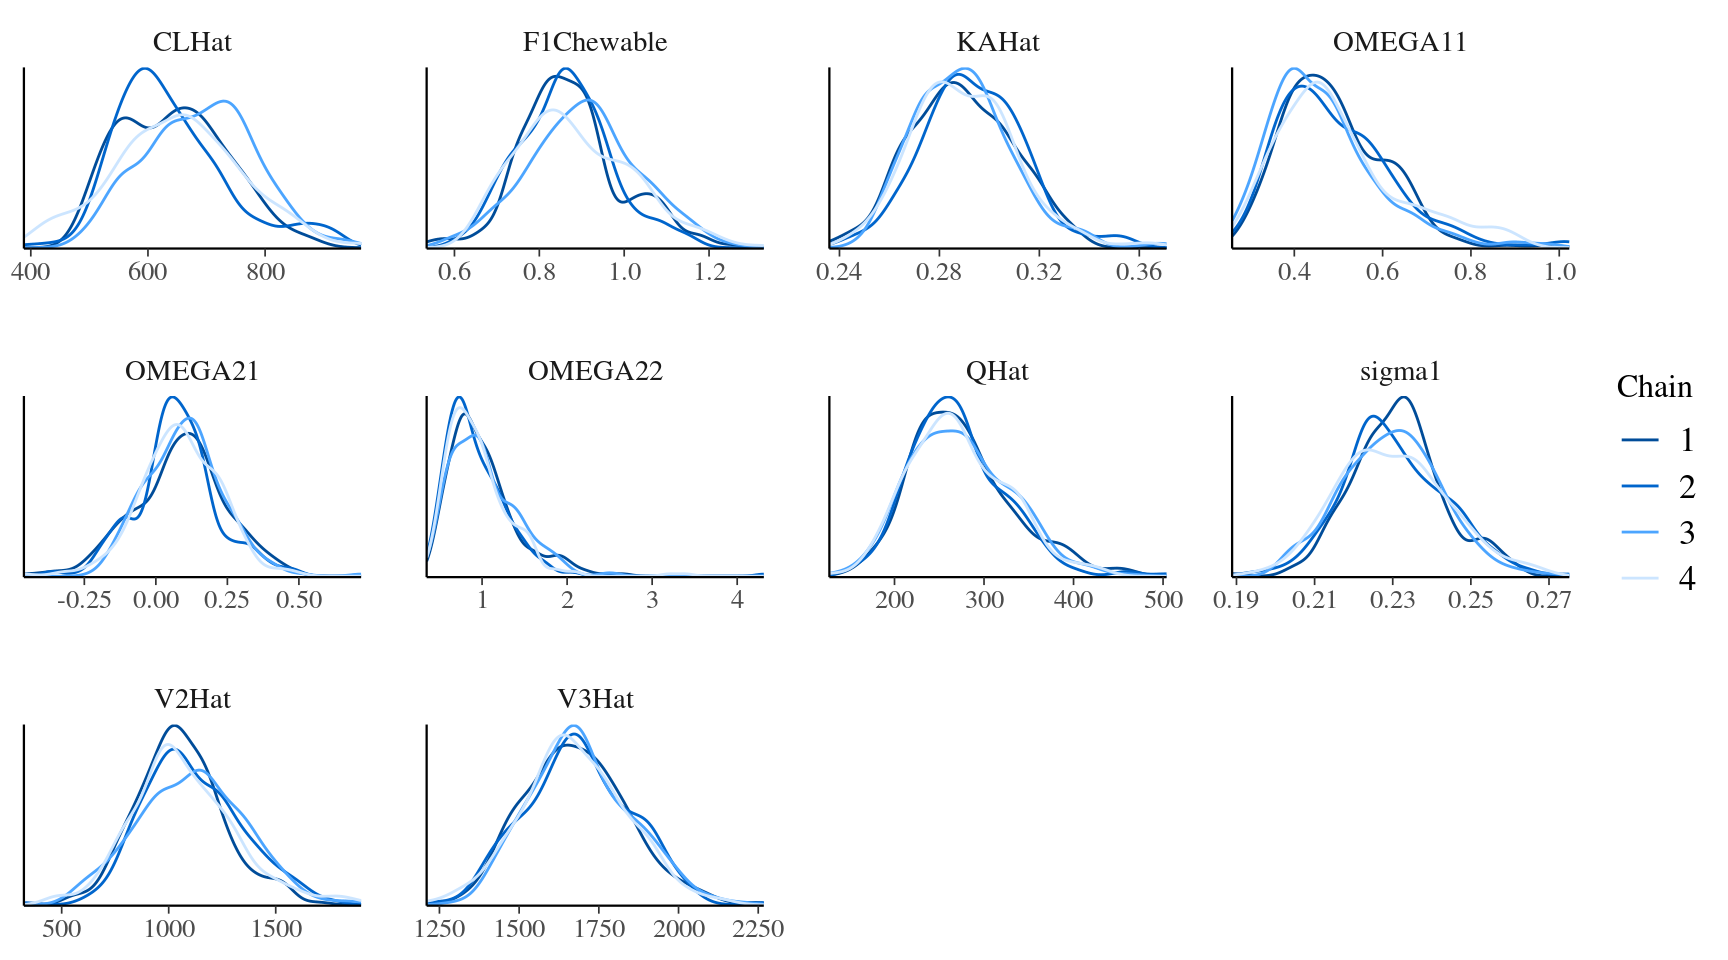
\includegraphics{/data/IntroBayesNONMEM/deliv/figure/atorv1/atorv1_parameters-3.pdf}
\caption{Pediatric atorvastatin PK example: Univariate marginal
densities by chain.}
\end{figure}

\begin{Shaded}
\begin{Highlighting}[]
\NormalTok{plot_mcmcDensity}
\end{Highlighting}
\end{Shaded}

\begin{verbatim}
. [[1]]
\end{verbatim}

\begin{figure}[htbp]
\centering
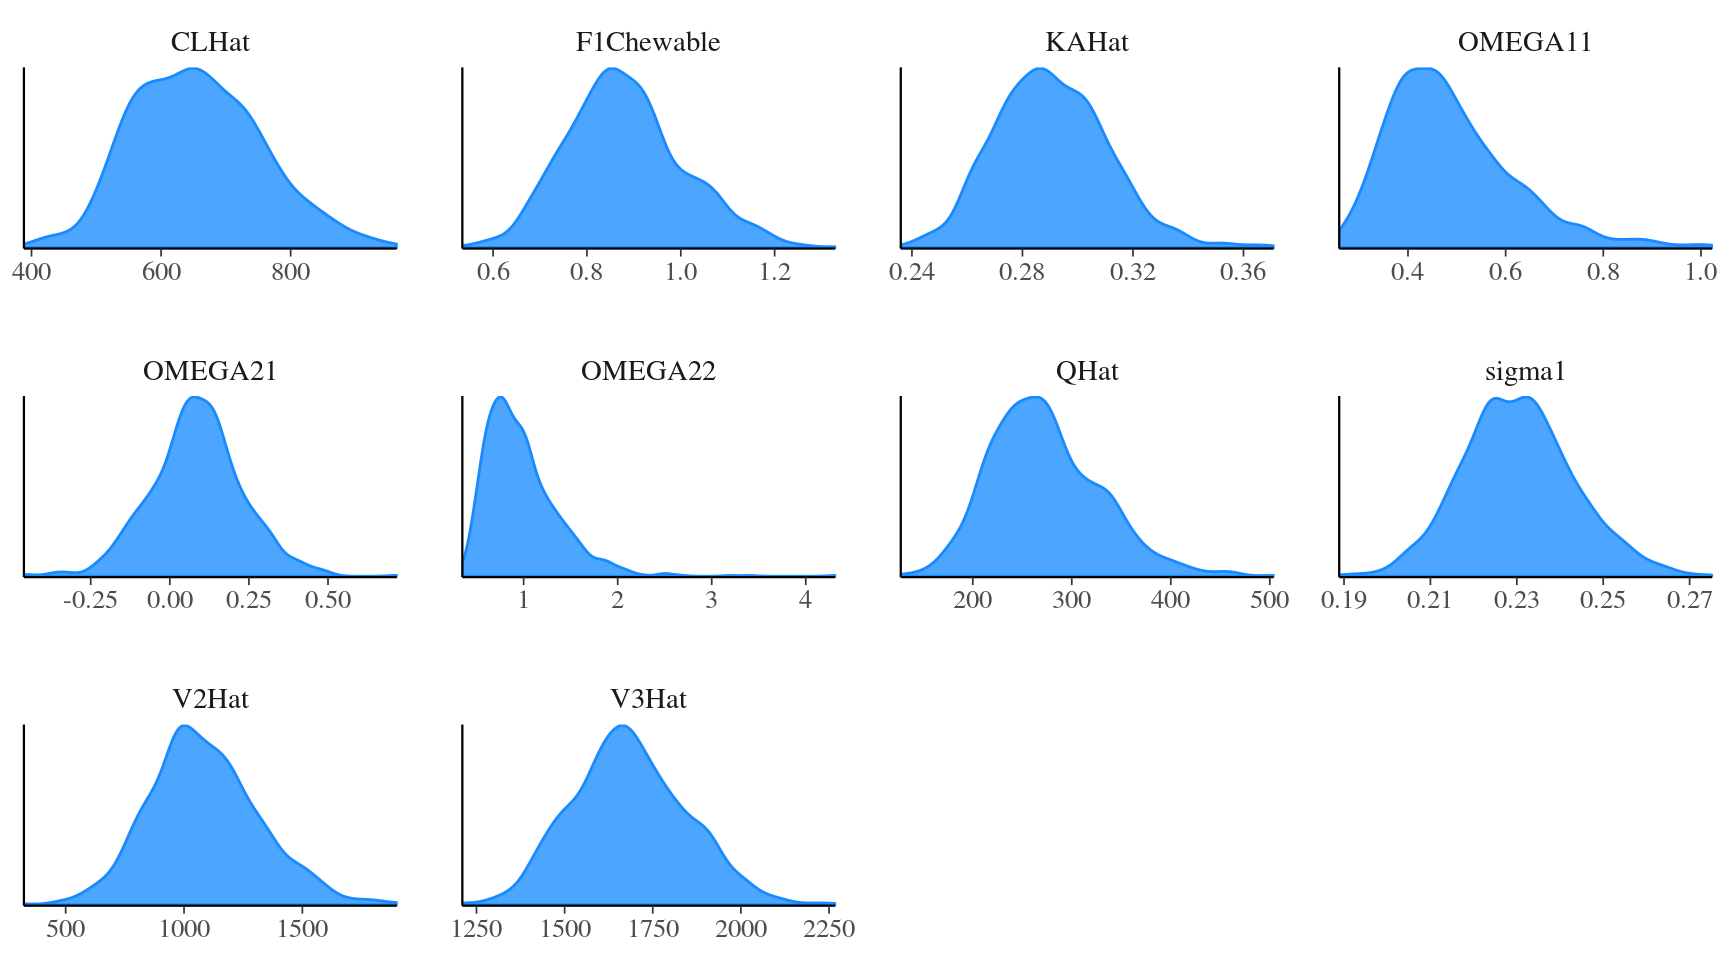
\includegraphics{/data/IntroBayesNONMEM/deliv/figure/atorv1/atorv1_parameters-4.pdf}
\caption{Pediatric atorvastatin PK example: Univariate marginal
densities.}
\end{figure}

\begin{Shaded}
\begin{Highlighting}[]
\KeywordTok{mcmc_pairs}\NormalTok{(popParArray)}
\end{Highlighting}
\end{Shaded}

\begin{figure}[htbp]
\centering
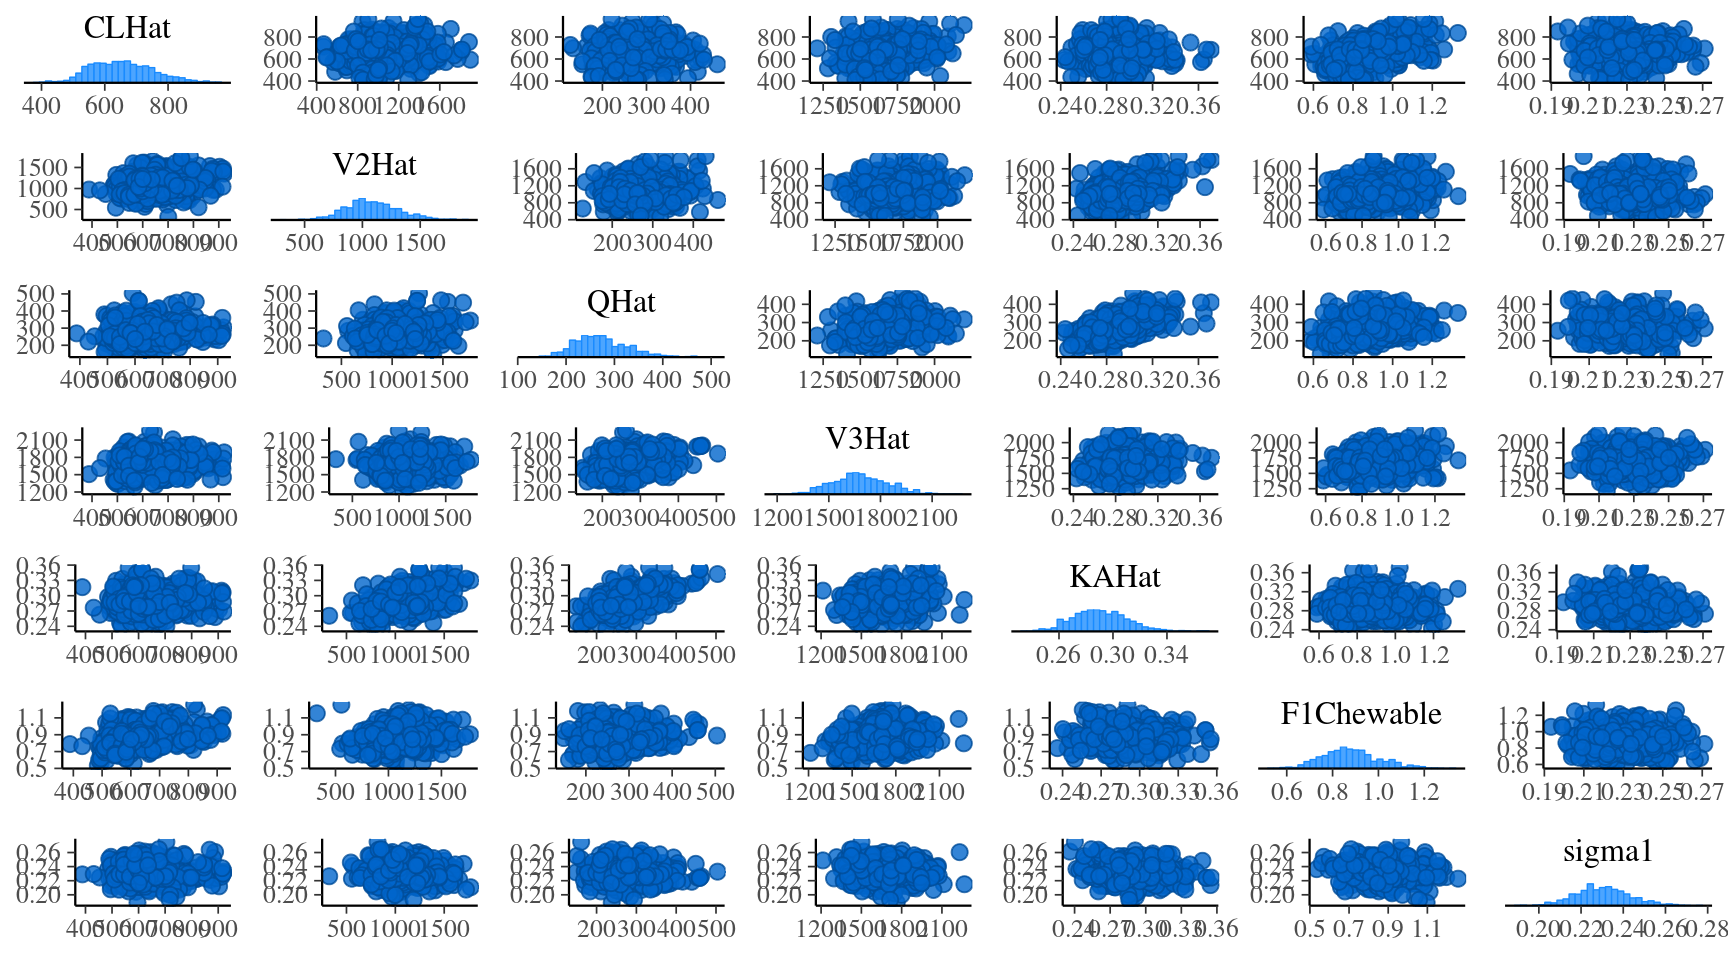
\includegraphics{/data/IntroBayesNONMEM/deliv/figure/atorv1/atorv1_parameters-5.pdf}
\caption{Pediatric atorvastatin PK example: Bivariate marginal
densities.}
\end{figure}

\begin{Shaded}
\begin{Highlighting}[]
\NormalTok{caption <-}\StringTok{ }\KeywordTok{paste}\NormalTok{(}\StringTok{"Pediatric atorvastatin PK example:"}\NormalTok{,}
      \KeywordTok{c}\NormalTok{(}\KeywordTok{rep}\NormalTok{(}\StringTok{"MCMC trace plots."}\NormalTok{, }\KeywordTok{length}\NormalTok{(plot_mcmcHistory)),}
        \KeywordTok{rep}\NormalTok{(}\StringTok{"Univariate marginal densities by chain."}\NormalTok{,}
            \KeywordTok{length}\NormalTok{(plot_mcmcDensityByChain)),}
        \KeywordTok{rep}\NormalTok{(}\StringTok{"Univariate marginal densities."}\NormalTok{,}
            \KeywordTok{length}\NormalTok{(plot_mcmcDensityByChain)),}
        \StringTok{"Bivariate marginal densities."}\NormalTok{)}
\NormalTok{)}

\NormalTok{ptable <-}\StringTok{ }\KeywordTok{monitor}\NormalTok{(popParArray, }
                  \DataTypeTok{warmup =} \DecValTok{0}\NormalTok{, }\DataTypeTok{print =} \OtherTok{FALSE}\NormalTok{) %>%}\StringTok{ }
\StringTok{  }\KeywordTok{formatC}\NormalTok{(}\DecValTok{3}\NormalTok{) %>%}
\StringTok{  }\NormalTok{as.data.frame}
\KeywordTok{write.csv}\NormalTok{(ptable, }\DataTypeTok{file =} \KeywordTok{file.path}\NormalTok{(tabDir, }\KeywordTok{paste}\NormalTok{(modelName, }
                                                 \StringTok{"ParameterTable.csv"}\NormalTok{, }\DataTypeTok{sep =} \StringTok{""}\NormalTok{)))}

\NormalTok{ptable %>%}\StringTok{ }
\StringTok{  }\KeywordTok{rename}\NormalTok{(}\DataTypeTok{SEmean =} \NormalTok{se_mean, }\DataTypeTok{SD =} \NormalTok{sd, }\DataTypeTok{pct2.5 =} \StringTok{"2.5%"}\NormalTok{, }\DataTypeTok{pct25 =} \StringTok{"25%"}\NormalTok{, }\DataTypeTok{median =} \StringTok{"50%"}\NormalTok{,}
         \DataTypeTok{pct75 =} \StringTok{"75%"}\NormalTok{, }\DataTypeTok{pct97.5 =} \StringTok{"97.5%"}\NormalTok{, }\DataTypeTok{Neff =} \StringTok{"n_eff"}\NormalTok{) %>%}
\StringTok{  }\KeywordTok{mutate}\NormalTok{(}\DataTypeTok{parameter =} \KeywordTok{rownames}\NormalTok{(.), }\StringTok{"95% CI"} \NormalTok{=}\StringTok{ }\KeywordTok{paste}\NormalTok{(}\StringTok{"("}\NormalTok{, pct2}\FloatTok{.5}\NormalTok{, }\StringTok{", "}\NormalTok{, pct97}\FloatTok{.5}\NormalTok{, }\StringTok{")"}\NormalTok{, }
                                                   \DataTypeTok{sep =} \StringTok{""}\NormalTok{)) %>%}
\StringTok{  }\KeywordTok{select}\NormalTok{(parameter, mean, SD, median, }\StringTok{"95% CI"}\NormalTok{, Neff, Rhat) %>%}
\StringTok{  }\KeywordTok{kable}\NormalTok{(}\DataTypeTok{caption =} \StringTok{"Summary of model parameter estimates."}\NormalTok{)}
\end{Highlighting}
\end{Shaded}

\begin{table}

\caption{\label{tab:parameters}Summary of model parameter estimates.}
\centering
\begin{tabular}[t]{l|l|l|l|l|l|l}
\hline
parameter & mean & SD & median & 95\% CI & Neff & Rhat\\
\hline
OMEGA11 & 0.307 & 0.0927 & 0.292 & (0.171, 0.531) & 288 & 1.02\\
\hline
OMEGA21 & -0.746 & 0.683 & -0.6 & (-2.54, 0.155) & 655 & 1.01\\
\hline
OMEGA22 & 17.4 & 16 & 12.2 & (2.92, 61.8) & 542 & 1.01\\
\hline
THETA1 & 7.06 & 0.123 & 7.06 & (6.81, 7.29) & 171 & 1.03\\
\hline
THETA2 & 5.72 & 1.19 & 5.88 & (3.02, 7.54) & 358 & 1.01\\
\hline
THETA3 & 4.94 & 0.346 & 4.96 & (4.19, 5.57) & 430 & 1.01\\
\hline
THETA4 & -1.92 & 0.0673 & -1.92 & (-2.04, -1.78) & 270 & 1.03\\
\hline
THETA5 & 7.32 & 0.14 & 7.32 & (7.04, 7.59) & 557 & 1.01\\
\hline
THETA6 & 0.77 & 0.165 & 0.754 & (0.479, 1.13) & 81 & 1.07\\
\hline
THETA7 & -0.968 & 0.0565 & -0.968 & (-1.08, -0.855) & 1.13e+03 & 1\\
\hline
\end{tabular}
\end{table}

\begin{Shaded}
\begin{Highlighting}[]
\KeywordTok{sessionInfo}\NormalTok{()}
\end{Highlighting}
\end{Shaded}

\begin{verbatim}
. R version 3.3.3 (2017-03-06)
. Platform: x86_64-pc-linux-gnu (64-bit)
. Running under: Ubuntu 14.04.5 LTS
. 
. locale:
.  [1] LC_CTYPE=en_US.UTF-8       LC_NUMERIC=C              
.  [3] LC_TIME=en_US.UTF-8        LC_COLLATE=en_US.UTF-8    
.  [5] LC_MONETARY=en_US.UTF-8    LC_MESSAGES=en_US.UTF-8   
.  [7] LC_PAPER=en_US.UTF-8       LC_NAME=C                 
.  [9] LC_ADDRESS=C               LC_TELEPHONE=C            
. [11] LC_MEASUREMENT=en_US.UTF-8 LC_IDENTIFICATION=C       
. 
. attached base packages:
. [1] parallel  grid      stats     graphics  grDevices utils     datasets 
. [8] methods   base     
. 
. other attached packages:
.  [1] bindrcpp_0.2.2       PKPDmisc_2.1.1       qapply_1.39         
.  [4] rlecuyer_0.3-4       knitr_1.20           kableExtra_0.9.0    
.  [7] gridExtra_2.3        forcats_0.3.0        stringr_1.3.1       
. [10] dplyr_0.7.7          purrr_0.2.5          readr_1.1.1         
. [13] tidyr_0.8.2          tibble_1.4.2         tidyverse_1.2.1     
. [16] bayesplot_1.6.0      rstan_2.14.1         StanHeaders_2.14.0-1
. [19] ggplot2_3.1.0        metrumrg_5.57        MASS_7.3-45         
. [22] XML_3.98-1.16        lattice_0.20-34      reshape_0.8.8       
. 
. loaded via a namespace (and not attached):
.  [1] Rcpp_0.12.19      lubridate_1.7.4   assertthat_0.2.0 
.  [4] rprojroot_1.3-2   digest_0.6.18     R6_2.3.0         
.  [7] cellranger_1.1.0  plyr_1.8.4        ggridges_0.5.1   
. [10] backports_1.1.2   stats4_3.3.3      evaluate_0.12    
. [13] highr_0.7         httr_1.3.1        pillar_1.3.0     
. [16] rlang_0.3.0.1     lazyeval_0.2.1    readxl_1.1.0     
. [19] data.table_1.11.8 rstudioapi_0.8    rmarkdown_1.10   
. [22] labeling_0.3      munsell_0.5.0     broom_0.5.0      
. [25] modelr_0.1.2      pkgconfig_2.0.2   htmltools_0.3.6  
. [28] tidyselect_0.2.5  viridisLite_0.3.0 crayon_1.3.4     
. [31] withr_2.1.2       nlme_3.1-128      jsonlite_1.5     
. [34] gtable_0.2.0      magrittr_1.5      scales_1.0.0     
. [37] cli_1.0.1         stringi_1.2.4     reshape2_1.4.3   
. [40] xml2_1.2.0        tools_3.3.3       glue_1.3.0       
. [43] hms_0.4.2         yaml_2.2.0        inline_0.3.14    
. [46] colorspace_1.3-2  rvest_0.3.2       bindr_0.1.1      
. [49] haven_1.1.2
\end{verbatim}

\end{document}
